
\documentclass{article}
\usepackage{cite}
\usepackage{amsmath,amssymb,amsfonts,amsthm}
\usepackage{algorithmic}
\usepackage{graphicx}
\usepackage{textcomp}
\usepackage{xcolor}
\usepackage{txfonts}
\usepackage{listings}
\usepackage{enumitem}
\usepackage{mathtools}
\usepackage{gensymb}
\usepackage[breaklinks=true]{hyperref}
\usepackage{tkz-euclide} % loads  TikZ and tkz-base
\usepackage{listings}
\usepackage[latin1]{inputenc}
       \usepackage{fullpage}
       \usepackage{color}
       \usepackage{array}
       \usepackage{longtable}
       \usepackage{calc}
       \usepackage{multirow}
       \usepackage{hhline}
       \usepackage{ifthen}
       \usepackage{multirow}
\usepackage{adjustbox}
\usepackage{hyperref}
\title{Audio Playlist Shuffler}
\author{Gitanshu Arora\\CS22BTECH11023}

\begin{document}

\maketitle

\section{Introduction}
The Audio Playlist Shuffler is a program designed to shuffle a playlist of songs and play them in a random order. The program utilizes various libraries and frameworks to provide a user-friendly interface for managing and playing the playlist.

\section{Methodology}
The following steps were involved in developing the Audio Playlist Shuffler:

\begin{enumerate}
    \item \textbf{Importing Dependencies}: The necessary libraries and frameworks were imported, including \texttt{numpy}, \texttt{tkinter}, \texttt{PIL}, and \texttt{pygame}. These libraries were chosen for their functionalities in handling arrays, creating graphical interfaces, and playing audio.
    
    \item \textbf{Playlist Generation}: An array of song IDs was generated to represent the playlist. The array was populated with sequential numbers representing the songs.
    
    \item \textbf{Shuffling the Playlist}: The \texttt{numpy} library was used to shuffle the array of song IDs, ensuring a random order for the playlist. The shuffled array was stored in a separate list for playback.
    
    \item \textbf{Interface Design}: The \texttt{tkinter} library was utilized to create a graphical interface for the Audio Playlist Shuffler. The interface included buttons for controlling playback (play/pause, next, previous) and a label to display the currently playing song.
    
    \item \textbf{Audio Playback}: The \texttt{pygame} library was employed to handle audio playback. The program loaded the audio files corresponding to the song IDs and played them based on user interactions with the interface. The program also implemented functionalities such as play/pause, next song, and previous song.
\end{enumerate}

\section{Results}
The Audio Playlist Shuffler successfully shuffles a playlist of songs and plays them in a random order. The program provides a user-friendly interface with buttons for controlling playback. The currently playing song is displayed in a label on the interface.

\section{Conclusion}
The development of the Audio Playlist Shuffler resulted in a functional program for managing and playing shuffled playlists of songs. The program's interface allows users to easily control playback and enjoy a randomized selection of songs from their playlist.

\section{Code}
The source code of the Audio Playlist Shuffler can be accessed through this \href{https://github.com/GitanshuA/AI-1110/blob/master/Audio%20Playlist%20Shuffler/main.py}{link}

\section{Images}
\begin{figure}[h]
\centering
    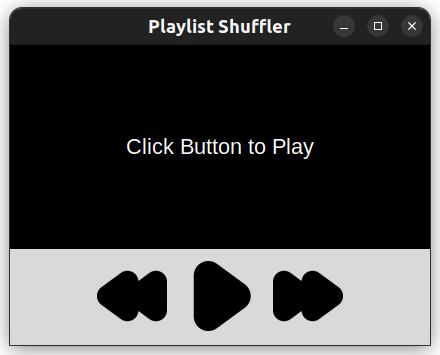
\includegraphics[width = 0.5\linewidth]{images/S.png}
    \caption{Initial State}
    \label{fig1}
\end{figure}
\begin{figure}[h]
\centering
    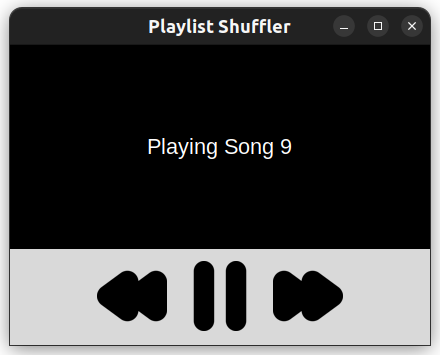
\includegraphics[width = 0.5\linewidth]{images/S1.png}
    \caption{Playing Music}
    \label{fig2}
\end{figure}

\end{document}
